
\documentclass[12pt]{article}

\usepackage[margin=1in]{geometry}
\usepackage{graphicx}
\usepackage{booktabs}
\usepackage{amsmath}
\usepackage{natbib}
\usepackage{setspace}

\onehalfspacing

\title{Replicating Figure 1 from Cavallo, Galiani, Noy, and Pantano (2013)}
\author{Ese Okitiakpe}
\date{\today}

\begin{document}

\maketitle

\section{Introduction}

This study replicates Catastrophic Natural Disasters and Economic Growth written by Cavallo, Galiani, Noy, and Pantano and published in Review of Economics and Statistics, 2013. The paper studies the causal effect of large natural disasters on economic growth\citep{cavallo2013}.

The contribution of this paper is that it gets around the following challenge: establishing a credible counterfactual for disaster-affected countries in the absence of a control group. It does this by constructing a synthetic control, a weighted combination of unaffected countries that closely matches the pre-disaster GDP trajectory of the treated country.

\section{Result of Interest}

This replication focuses on Figure 1, ``Increasing Prevalence of Natural Disasters 1970--2007,'' from Cavallo et al. (2013). The figure reports the annual number of recorded natural disaster events worldwide and the annual number of large disasters, defined as events whose intensity exceeds the mean of the normalized killed distribution.

This result is important because it provides evidence that the observed increase in recorded natural disasters over time is primarily driven by improved reporting of smaller events rather than an increase in truly catastrophic disasters. The figure serves as a key motivation for the paper's broader analysis of the economic consequences of large natural disasters and helps justify the use of more sophisticated empirical methods in the remainder of the study.


\section{Data}

The data are from the EM-DAT database (Centre for Research on the Epidemiology of Disasters, Catholic University of Louvain) and contain information on the occurrence, type, and magnitude of natural disasters worldwide, including the number of people killed, affected, and the estimated economic damage. The sample includes 6,530 disaster events across 196 countries covering the period 1970-2008.

The data were originally collected by the Centre for Research on the Epidemiology of Disasters (CRED) at the Catholic University of Louvain, and are publicly available at www.cred.be. The key variables used in the replication are the year of the disaster event, the type of disaster (earthquake, storm, or flood), the number of people killed normalized by population, and a binary indicator for whether the event qualifies as a large disaster based on the world pooled mean of the killed distribution.

The original code is written in Stata 16.1 and this replication reproduces the analysis in Stata 14.2, using the descriptives-REPLIC.do file from the authors' publicly available replication package on the Harvard Dataverse |\textbf{(doi:10.7910/DVN/26717)}.

\section{Methods}

The primary method is descriptive time series analysis using the EM-DAT disaster database, which does the following: for each year from 1970 to 2007, the code counts the total number of recorded natural disaster events and separately counts the number of large events defined as those whose intensity (measured by people killed as a share of population) exceeds the world pooled mean. These two series are plotted on a dual-axis time series chart, with total events on the left axis and large events on the right axis, to show that while disaster recording has increased over time, truly catastrophic events have not.

Because Figure 1 is a descriptive result, no causal parameter is estimated. Instead, the figure summarizes annual trends in the frequency of natural disaster events and large disaster events over time.

The core estimating equation of the paper is the factor model underlying the synthetic control method (Equation 4 in the original paper):

\begin{equation}
Y^N_{it} = \delta_t + \theta_t Z_i + \lambda_t \mu_i + \varepsilon_{it}
\end{equation}

where:
\begin{itemize}
    \item $Y^N_{it}$ is the real GDP per capita that would be observed for country $i$ at time $t$ in the absence of a natural disaster
    \item $Z_i$ is a vector of observed predictors for GDP per capita not affected by the natural disaster, including trade openness, capital stock, land area, population, education, latitude, and political institutions
    \item $\lambda_t \mu_i$ is a vector of unobserved common factors $\lambda_t$ multiplied by unknown factor loadings $\mu_i$, capturing time-varying confounders
    \item $\varepsilon_{it}$ is a transitory GDP per capita shock with zero mean
\end{itemize}

While Figure 1 is a descriptive result, this equation motivates the paper's causal identification strategy used in subsequent figures.

The replication was implemented using two R scripts. The preprocessing script, \texttt{preprocess.R}, reads the original EM-DAT disaster dataset, constructs the normalized deaths-per-population measure (\texttt{killed\_pop}), filters disaster observations, and produces an analysis-ready dataset.

The analysis script, \texttt{analysis.R}, uses the processed data to identify large disasters as events with intensity above the mean normalized killed distribution. It then aggregates disaster events by year and reproduces Figure~1 from \citet{cavallo2013}.

Finally, the script exports the replicated figure and automatically generates the corresponding \LaTeX{} table fragment used in the paper.


\section{Replication Results}

The following figure replicates Figure 1 from Cavallo et al. (2013), showing the increasing prevalence of natural disaster events from 1970 to 2007.


\begin{figure}[h]
    \centering
    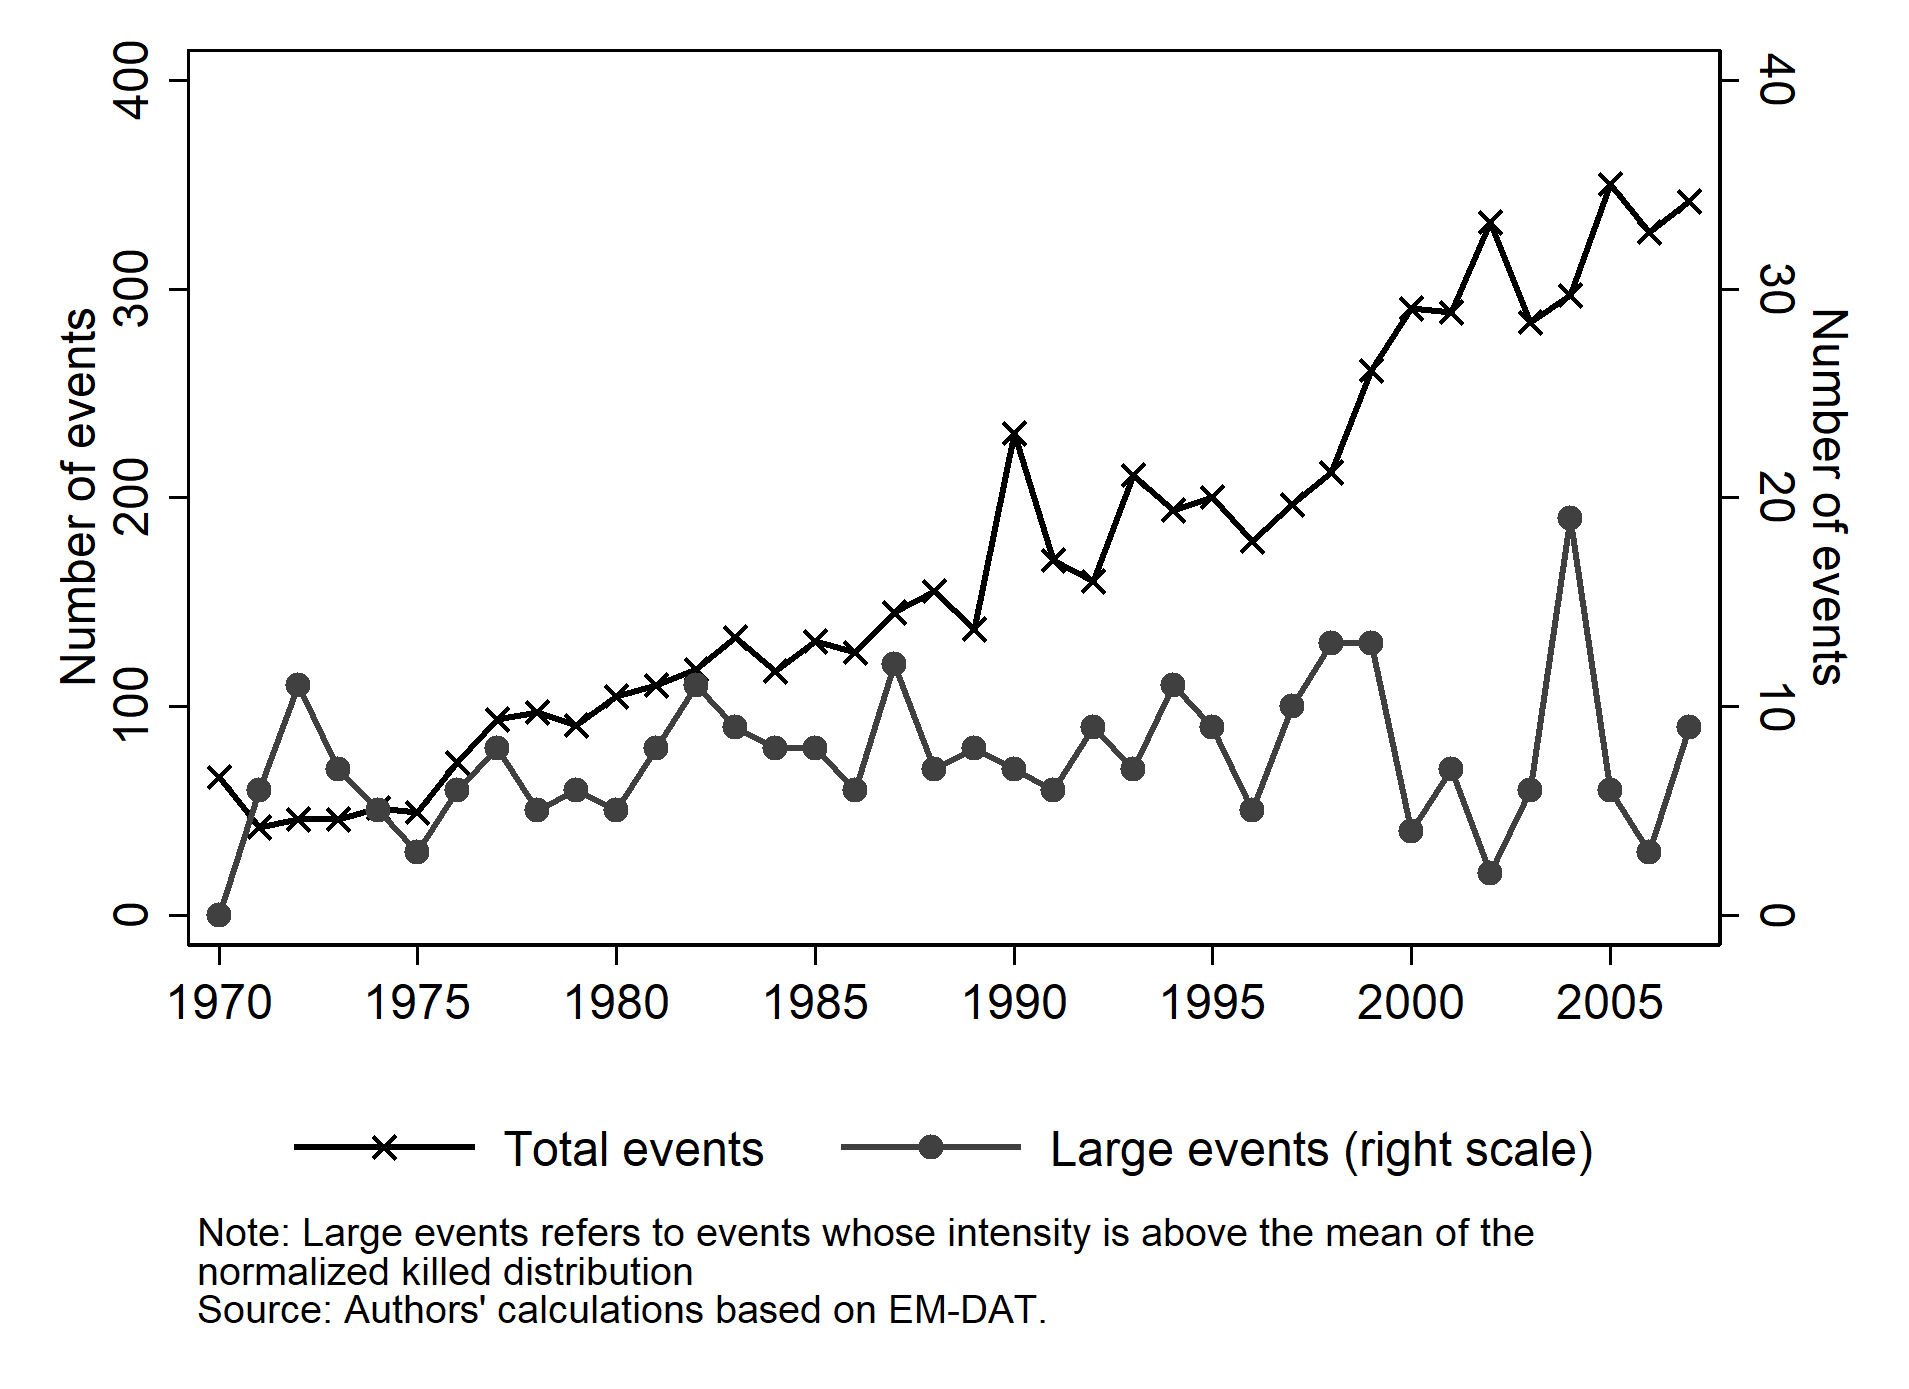
\includegraphics[width=0.75\textwidth]{figures/fig1.png}
    \caption{Increasing Prevalence of Natural Disasters 1970--2007. Replication of Figure 1 from Cavallo et al. (2013). Note: Large events refers to events whose intensity is above the mean of the normalized killed distribution. Source: Authors' calculations based on EM-DAT.}
\end{figure}

The main finding is that while total recorded disaster events increased steadily from roughly 70 per year in 1970 to over 300 per year by 2007, the number of truly large disasters those above the mean of the normalized killed distribution remained relatively stable throughout the period.
This result tells us in plain English that the apparent increase in natural disasters is driven by improved recording of minor events, not by an increase in catastrophic ones. Large disasters are relatively rare compared to the total number of recorded disaster events, which helps explain why the authors later employ more sophisticated methods to study their economic effects.

Compared to the original paper, the replicated figure closely matches the published result. The original figure shows that the total number of recorded natural disaster events increased substantially between 1970 and 2007, while the number of large disasters remained relatively stable over the same period.

The replication reproduces the same pattern. In the replicated figure, total events increase from 66 events in 1970 to 342 events in 2007, whereas large events fluctuate around a relatively stable level. The qualitative conclusion is therefore identical to that reported by Cavallo et al. (2013): the observed increase in recorded disasters appears to be driven primarily by improved reporting and recording of smaller events rather than an increase in truly catastrophic disasters.


\section{Challenges in Replication}

The challenges in replicating the results were the following:

\begin{itemize}
    \item The \texttt{synth} package for Stata was not available on SSC and could not be installed on Windows 64-bit due to a missing plugin file (\texttt{synthopt.win64a}), preventing replication of the main synthetic control figures (Figures 3, 9, 10).
    \item The sovereign bond spread data used in related papers was proprietary (Bloomberg), illustrating how data availability constraints frequently limit replication even when code is publicly posted.
    \item The replication package README noted that computation takes approximately 4 hours, highlighting the computational burden of synthetic control methods with large donor pools.
    \item An alternative R implementation using the \texttt{Synth} package produced a qualitatively similar synthetic control estimate for Nicaragua but required a balanced panel and reduced predictor set due to missing covariate data in early years (1960--1967).
\end{itemize}

One important lesson from the replication process is that software dependencies and package availability are a major barrier to reproducibility, even when code and data are publicly posted. The \texttt{synth} package failure on Windows 64-bit meant the core results of the paper could not be replicated without significant additional effort.

\section{What I Learned}

The replication process highlighted how software dependencies can become a major barrier to reproducibility. Although the authors provided code and data, the synth package for Stata could not be installed on Windows 64-bit because of a missing plugin file. As a result, some of the paper's synthetic control figures could not be reproduced directly.

I also learned that data availability remains a challenge in empirical economics. While Figure 1 relied on publicly available EM-DAT data, other analyses often depend on proprietary datasets that are difficult for researchers to access.

The easiest part of the replication was reproducing Figure 1 because the required data and code were publicly available. The most difficult part was understanding the software requirements and reproducing results that relied on specialized Stata packages.

Overall, this exercise demonstrated that making code public is important but not always sufficient for reproducibility. Software compatibility, documentation quality, and data accessibility are equally important.

\section{Takeaways}

The following would be the main takeaways of the paper:

\begin{enumerate}
    \item Truly catastrophic natural disasters those above the 99th percentile of the killed distribution are extremely rare, with only 4 events qualifying in the 1970--2000 sample period.
    \item The rarity of large disasters makes synthetic control the appropriate causal identification strategy, since standard panel regression requires many treated units.
    \item Even extremely large natural disasters do not significantly affect long-run GDP growth unless they are followed by radical political revolution, as in Nicaragua (1979) and Iran (1979).
\end{enumerate}

Overall, the paper contributes to the literature by providing the first rigorous causal evidence that natural disasters alone do not harm long-run economic growth; rather, it is the political instability that sometimes follows disasters that drives negative outcomes.

\section{Extensions}

The following would be possible extensions of the paper:

\begin{itemize}
    \item Extending the sample to post-2000 disasters, including the 2004 Indian Ocean Tsunami and the 2010 Haiti earthquake, using updated EM-DAT data.
    \item Applying the synthetic control method to climate-related disasters specifically, to assess whether the results hold for slow-onset events like droughts.
    \item Replicating the analysis using the \texttt{Synth} package in R with a fully balanced panel to assess robustness to software implementation differences.
\end{itemize}

Future work could also explore whether the null effect of natural disasters on growth holds in the post-2000 period, given the increasing frequency of climate-related disasters and improvements in international disaster response.

\bibliographystyle{apalike}
\bibliography{references}

\end{document}
